% !TEX root = B&G_oefeningen.tex
\chapter{Binary min-heap}
\section*{Inleiding}

Download het bestand \verb=week05-06_Heap.zip= van Toledo. Ontzip het. Om de broncode van de oefeningen in IntelliJ te krijgen: map NIET openen, wel code IMPORTEREN (File > New > Project from Existing Sources of bij beginscherm: “import project”). 



\begin{oef}
\papier Gegeven twee binaire bomen in figuren~\ref{fig:arrayimpl1} en \ref{fig:arrayimpl2} op pagina~\pageref{fig:arrayimpl2}. Stel dat je intern een arrayimplementatie voor bomen gebruikt. Welke array zou je dan bekomen voor deze beide bomen?
\begin{figure}[p]
    \centering
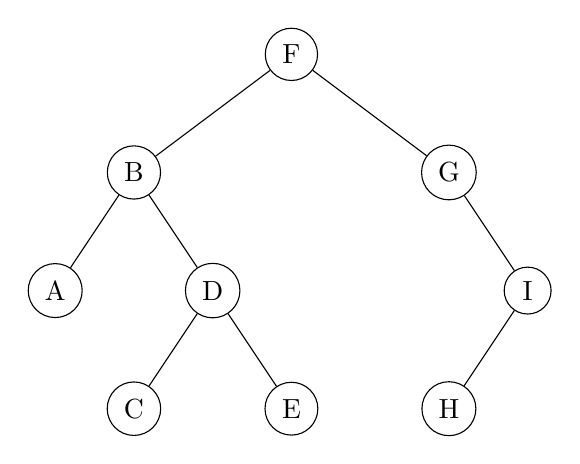
\begin{tikzpicture}[every node/.style={circle,draw},
				level 1/.style={sibling distance=40mm},
				level 2/.style={sibling distance=20mm}]
\node {F}
child { node {B} 
	child { node {A} }
	child { node {D} 
		child { node {C} } 
		child { node {E} } }
}
child { node {G}
	child[missing]
	child { node {I}
		child { node {H}}
		child[missing]}};
\end{tikzpicture}
\caption{Welke arrayimplementatie voor deze binaire boom?}
    \label{fig:arrayimpl1}
\end{figure}

\begin{figure}[p]
    \centering
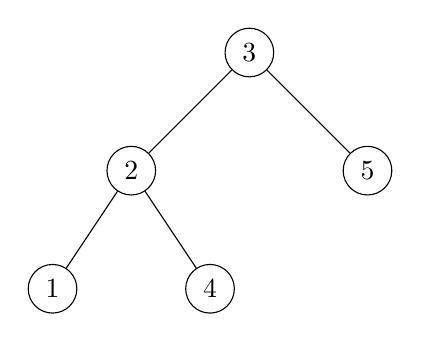
\begin{tikzpicture}[every node/.style={circle,draw},
				level 1/.style={sibling distance=30mm},
				level 2/.style={sibling distance=20mm}]
\node {3}
child { node {2} 
	child { node {1} }
	child { node {4} }
}
child { node {5}};
\end{tikzpicture}
\caption{Hoe deze boom voorstellen met een array?}
    \label{fig:arrayimpl2}
\end{figure}
\begin{opl}
Zoals we in de theorie zagen, moet je een bepaalde waarde afspreken om aan te geven dat een bepaald kind ontbreekt. Laten we dat voor de eenvoud hier gewoon voorstellen door het getal \verb+0+.
Een mogelijke arrayimplementatie voor figuur~\ref{fig:arrayimpl1} is:\\
\verb+[F, B, G, A, D, 0, I, 0, 0, C, E, 0, 0, H]+ \\
Voor figuur~\ref{fig:arrayimpl2}: \verb+[3, 2, 5, 1, 4]+. Aangezien dit een complete binaire boom is, bevat de array geen “nullen”.
\end{opl}

\end{oef}


\begin{oef}
\papier Een gegeven binaire min-heap bevat 1000 knopen. Intern wordt deze met een array voorgesteld.
\begin{oefenumerate}
	\item Waar vind je de ouder van de knoop die zich in de array op index 256 bevindt?
	\item Waar vind je de rechterbuur (op hetzelfde niveau) van de knoop die zich in de array op index 72 bevindt? Op welk niveau staan die beiden? Hebben die beiden dezelfde ouder?
	\item Heeft de knoop die zich in de array op index 249 bevindt kleinkinderen?
\end{oefenumerate}
\begin{opl}
Een goed startpunt om deze oefening op te lossen is een tekening maken. Het lukt natuurlijk niet om heel de boom te tekenen, maar we kunnen wel de eerste niveau's tekenen en dan de kracht van abstractie toepassen op zoek naar een patroon.

Bekijk figuur~\ref{fig:1000knopen}. Op niveau 1 is er één knoop met nummer 0. Op niveau 2 zijn er twee knopen, nummer 1 en 2. Als we deze getallen in een tabel zetten (tabel~\ref{tbl:1000knopen}) valt er één en ander op.
\begin{figure}[htbp]
    \centering
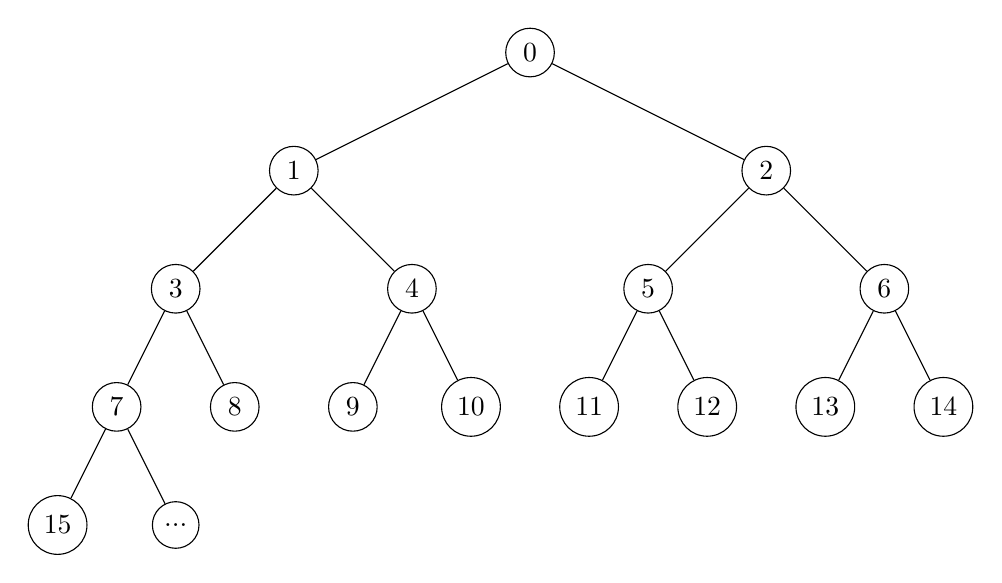
\begin{tikzpicture}[every node/.style={circle,draw},
				level 1/.style={sibling distance=60mm},
				level 2/.style={sibling distance=30mm},
				level 3/.style={sibling distance=15mm}]
\node {0}
child { node {1} 
	child { node {3}
		child { node {7} 
			child {node {15}}
			child {node {...}}
		}
		child { node {8} }
	 }
	child { node {4} 
		child { node {9} }
		child { node {10} }
		}
}
child { node {2}
	child { node {5}
		child { node {11} }
		child { node {12} }
	 }
	child { node {6} 
		child { node {13} }
		child { node {14} }
	}
};
\end{tikzpicture}
\caption{Op weg naar 1000 knooppunten, genummerd van 0 tot 999}
    \label{fig:1000knopen}
\end{figure}

\begin{table}[ht]
  \centering
  \caption{Overzicht van alle knopen}
  \begin{tabular}{rrrr}
    \toprule 
niveau & aantal & nummers & totaal \\
\midrule
1 & 1 & 0 & 1\\
2 & 2 & $1 \rightarrow 2$ & 3\\
3 & 4 & $3 \rightarrow 6$ & 7\\
4 & 8 & $7 \rightarrow 14$ & 15\\
5 & 16 & $15 \rightarrow 30$ & 31\\
... & ... & ... & ...\\
$i$ & $2^{i-1}$ & $2^{i-1}-1 \rightarrow 2^i-2$ & $2^i - 1$\\
... & ... & ... & ...\\
9 & 256 & $255 \rightarrow 510$ & 511\\
\bottomrule
  \end{tabular}
  \label{tbl:1000knopen}
\end{table}
Op niveau 9 zijn er dus 256 knooppunten, genummerd van 255 tot 510. In totaal heeft deze binaire boom op de eerste 9 niveau's samen 511 elementen. Op niveau 10 zou er plaats zijn voor 512 elementen, maar dat hoeft niet meer. Als er in totaal 1000 knooppunten moeten zijn, zal het laagste niveau nog $1000-511=489$ knopen tellen.

Met deze informatie kunnen we nu de vragen beantwoorden:
\begin{oefenumerate}
	\item \emph{Waar vind je de ouder van de knoop die zich in de array op index 256 bevindt?} De knoop met nummer 256 staat op niveau 9 als tweede van links. Het is het rechterkind van de knoop op niveau 8 met nummer 127. Dat is de eerste knoop links op het achtste niveau.
	\item \emph{Waar vind je de rechterbuur (op hetzelfde niveau) van de knoop die zich in de array op index 72 bevindt?} Knoop 72 bevindt zich op niveau 7, meerbepaald de tiende knoop op dit niveau. De rechterbuur van 72 is natuurlijk knoop 73. Beide knopen hebben een verschillende ouder (welke?).
	\item \emph{Heeft de knoop die zich in de array op index 249 bevindt kleinkinderen?} De kinderen van knoop $i$ zijn knopen $2i+1$ en $2i+2$. Knoop 249 heeft dus twee kinderen: 499 en 500. De kinderen van 499 zijn nummer 999 en 1000, die van 500 zijn 1001 en 1002. Vermits deze boom maar duizend knopen heeft, heeft de laatste knoop het nummer 999. Daaruit volgt dat knoop 249 wel degelijk één kleinkind heeft, nl. de allerlaatste knoop op het tiende niveau rechts, met nummer 999.
\end{oefenumerate}
\end{opl}

\end{oef}


\begin{oef}
\code De \verb=BinaryMinHeap= klasse bevat 1 instantievariabele: \verb=values=, een arraylist die de waarden van de min-heap bevat. Hierbij zal in het eerste element van de arraylist steeds de kleinste waarde van de values zitten.

Voeg een methode \verb=getMin= aan de \verb=BinaryMinHeap= klasse toe die de minimale waarde opgeslagen in de min-heap teruggeeft.	De methode gooit een \verb+IllegalStateException+ indien de heap geen elementen bevat. Voor het testen van deze methode moet je even wachten tot na de implementatie van de \verb+addValue+ methode in de volgende oefening.
\begin{opl}
\begin{lstlisting}[caption={kleinste waarde van min-heap}, label=minheapkleinste]
public E getMin() {
	if (this.values.size() == 0) {
		throw new IllegalStateException();
	} else {
		return this.values.get(0);
	}
}
\end{lstlisting}

\end{opl}

\end{oef}


\begin{oef}
\code In deze oefening bekijken we het toevoegen van een gegeven waarde aan een min-heap.
\begin{oefenumerate}
	\item Bestudeer de methode \verb=addValue= van de \verb=BinaryMinHeap= klasse die een gegeven waarde aan de min-heap toevoegt. Zie de slides van deze les voor meer uitleg.
	\item Implementeer de \verb=bubbleUp= functie in de \verb=BinaryMinHeap= klasse.
	\item Run de \verb=main= functie in de \verb=BinaryMinHeapDriver= klasse en controleer hiermee de implementatie van de \verb=addValue= en \verb=getMin= methode. \newline Verwachte uitvoer : \newline [-7, -4, -2, 0, 1, 2, -1, 3, 2] \newline Kleinste waarde = -7
\end{oefenumerate}
\begin{opl}
\begin{lstlisting}[caption={bubbleUp methode}, label=minheapbubbleUp]
private void bubbleUp() {
	int index = this.values.size() - 1; //start met laatste element
		
	while (heeftOuder(index) && ouder(index).compareTo(values.get(index)) > 0) {
		//ouder en kind staan in verkeerde volgorde, wissel ze om
		this.wisselOm(index, ouderIndex(index));
		index = ouderIndex(index);
	}
}

private boolean heeftOuder(int i) {
	return i >= 1;
}

private E ouder(int i) {
	return values.get(ouderIndex(i));
}

private int ouderIndex(int i) {
	return (i - 1)/2;
}
	
private void wisselOm(int i, int j) {
	//wissel i-de en j-de element in de ArrayList om
	E hulp = this.values.get(i);
	this.values.set(i, this.values.get(j));
	this.values.set(j, hulp);
}
\end{lstlisting}
\end{opl}
\end{oef}




\begin{oef}
\code Deze oefening gaat over het verwijderen van het kleinste getal uit een binary min-heap.
\begin{oefenumerate}
	\item Bestudeer de methode \verb=removeSmallest= van de \verb=BinaryMinHeap= klasse die een gegeven waarde uit de min-heap verwijdert. Zie de slides van deze les voor meer uitleg.
	\item Implementeer de \verb=bubbleDown= functie in de \verb=BinaryMinHeap= klasse.
	\item Run de \verb=main= functie in de \verb=BinaryMinHeapDriver= klasse en controleer hiermee de implementatie van de \verb=removeSmallest= methode. \newline Verwachte uitvoer: \newline
-7 \newline
[-4, 0, -2, 2, 1, 2, -1, 3] \newline
-4 \newline
[-2, 0, -1, 2, 1, 2, 3] \newline
-2 \newline
[-1, 0, 2, 2, 1, 3] \newline
-1 \newline
[0, 1, 2, 2, 3] \newline
0 \newline
[1, 2, 2, 3]
\end{oefenumerate}
\begin{opl}
\begin{lstlisting}[caption={bubbleDown methode}, label=minheapbubbleDown]
private void bubbleDown() {
	int index = 0; //start met de wortel
		
	boolean wisselOK = true;
	while (heeftLinkerKind(index) && wisselOK) {
		//welk kind is het kleinste?
		int indexKleinsteKind = indexLinkerKind(index);
		if (heeftRechterKind(index)
			&& values.get(indexKleinsteKind).compareTo(values.get(indexRechterKind(index))) > 0) {
			indexKleinsteKind = indexRechterKind(index);
		}
		//vergelijk ouderwaarde met waarde van kleinste kind
		if (values.get(index).compareTo(values.get(indexKleinsteKind)) > 0) {
			//foute volgorde, wissel om				
			this.wisselOm(index, indexKleinsteKind);
		} else {
			//volgorde OK, while lus mag stoppen
			wisselOK = false;
		}
			
		//vertrek nu vanuit de index van het kleinste kind
		index = indexKleinsteKind;
	}
}

private int indexLinkerKind(int i) {
	return 2 * i + 1;
}
	
private int indexRechterKind(int i) {
	return 2 * i + 2;
}
	
private boolean heeftLinkerKind(int i) {
	return indexLinkerKind(i) < values.size();
}
	
private boolean heeftRechterKind(int i) {
	return indexRechterKind(i) < values.size();
}
\end{lstlisting}

\end{opl}

\end{oef}

\begin{oef}
\code In een binary min-heap is elk pad van de kleinste naar een ander element gesorteerd. 

\begin{oefenumerate}
	
	\item Implementeer een \verb=getPath= functie in de \verb=BinaryMinHeap= klasse die het pad van de kleinste naar een gegeven dataveld geeft indien mogelijk.
	\item Run de \verb=main= functie in de \verb=BinaryMinHeapDriver= klasse en controleer hiermee de implementatie van de \verb=getPath= methode. \newline Verwachte uitvoer : \newline [1, 2, 3] \newline
[1, 2] \newline
null
\end{oefenumerate}
\begin{opl}
\begin{lstlisting}[caption={getPath methode}, label=minheapgetPath]
public ArrayList<E> getPath(E value) {
	int index = this.values.indexOf(value);
	if (index == -1) {
		//value komt niet voor in de heap
		return null;
	} else {
		//value zit in heap, index = plaats van eerste voorkomen
		ArrayList<E> pad = new ArrayList<>();
		pad.add(value);
		while (index > 0) {
			//we zijn nog niet aan de wortel
			index = (index - 1)/2; //ouder
			pad.add(0, this.values.get(index)); //voeg vooraan toe
		}
	return pad;	
	}
}
\end{lstlisting}
\end{opl}

\end{oef}


